% Số liệu lịch sử từ benchmarks/benchmark_20_maps.csv, không phải đo lại main.
\section{Benchmark và trực quan hóa kết quả}
\label{sec:benchmark}

\subsection{Thiết kế phép đo}

Bộ dữ liệu được xây dựng trong giai đoạn tích hợp UI gồm 20 maps,
4 thuật toán và 1 lần chạy cho mỗi cặp, tổng cộng 80 lượt. Mỗi lượt dùng
trạng thái khởi tạo của map và cùng bộ luật chơi. Mã nguồn được đo là
commit \texttt{29f2323}; môi trường được ghi nhận là Python 3.14.7,
macOS 26.6.2 trên ARM64. Dữ liệu và phương pháp được lưu trong
\path{benchmarks/benchmark_20_maps.csv} và tài liệu schema đi kèm
\cite{bloxorz_benchmark_data}.

Đây là kết quả của phiên bản lịch sử, không phải số đo mới của
\texttt{main} hiện tại. Repository hiện có thêm 15 maps và dữ liệu riêng;
phần phân tích này giữ phạm vi 20 maps ban đầu, không gộp các đợt đo có
phiên bản code khác nhau. Đặc biệt, cách cài đặt DFS đã thay đổi khi tích
hợp với \texttt{main}, nên không dùng CSV cũ để khẳng định hiệu năng của
DFS hiện tại.

Các lượt chạy được thực hiện tuần tự theo map01 đến map20, trong mỗi map
theo thứ tự BFS, DFS, UCS, A*. Mỗi lượt tạo bàn cờ và tiến trình
\texttt{spawn} mới. Giới hạn nội bộ là 30 giây và 150.000 node mở rộng;
tiến trình cha dùng deadline 35 giây, kể cả khởi động worker.

\texttt{Benchmark} đo cả kiểm tra đầu vào, khởi tạo solver và tìm kiếm,
bao gồm dựng bảng heuristic của A*. Phép đo không bao gồm đọc map,
khởi động tiến trình, vẽ UI, truyền kết quả hoặc replay kiểm chứng.
Các đại lượng được sử dụng như sau:
\begin{itemize}
    \item Thời gian: chênh lệch \texttt{perf\_counter}, đơn vị giây, có
    overhead của cơ chế theo dõi bộ nhớ.
    \item Bộ nhớ: đỉnh cấp phát Python do \texttt{tracemalloc} theo dõi,
    không phải tổng RAM/RSS của tiến trình; khi vẽ đổi byte sang MiB
    bằng cách chia cho $2^{20}$.
    \item Node mở rộng: số node thực sự sinh successors; không tính
    node đích, heap entry cũ hoặc tiền xử lý heuristic.
    \item Chất lượng lời giải: số hành động và tổng chi phí. Hai giá trị
    bằng nhau vì mọi hành động đều có chi phí 1.
\end{itemize}

\subsection{Schema CSV và kiểm chứng dữ liệu}

Schema phiên bản \texttt{1.0.0} có 21 cột cố định, mỗi dòng biểu diễn một
lượt chạy. Khóa duy nhất là
\texttt{(run\_id, map\_id, algorithm, trial)}. Các cột được nhóm theo
vai trò để tiện trình bày trong Bảng~\ref{tab:csv_groups}; tên, thứ tự
và kiểu đầy đủ nằm trong \path{docs/benchmark_csv_schema.md}.

\begin{table}[htbp]
    \centering
    \caption{Các nhóm thông tin trong schema benchmark}
    \label{tab:csv_groups}
    \small
    \begin{tabularx}{\textwidth}{@{}p{3.3cm}X@{}}
        \toprule
        \textbf{Nhóm} & \textbf{Thông tin lưu trữ} \\
        \midrule
        Nhận diện lượt đo & Phiên bản schema, run ID, thời điểm, map,
        thuật toán, số thứ tự lần chạy. \\
        Nguồn và môi trường & Commit Git, phiên bản Python, nền tảng,
        SHA-256 của file maps. \\
        Kết quả và giới hạn & Trạng thái, thời gian, bộ nhớ, số node,
        giới hạn thời gian và giới hạn node. \\
        Lời giải và kiểm chứng & Độ dài, chi phí, chuỗi hành động,
        cờ replay hợp lệ và thông báo. \\
        \bottomrule
    \end{tabularx}
\end{table}

Ô trống của trường nullable biểu diễn dữ liệu không có, không thay bằng
0. Chỉ khi \texttt{status=solved} mới có độ dài và chi phí lời giải.
Trạng thái \texttt{limit} không chứng minh map vô nghiệm.

Sau mỗi lượt giải, chuỗi hành động được replay độc lập ngoài khoảng đo
bằng \texttt{apply\_action()} và kiểm tra kết thúc bằng
\texttt{is\_goal()}. Bộ dữ liệu có đủ 80 khóa duy nhất, 80 lượt
\texttt{solved} và 80 lời giải replay hợp lệ. Notebook kiểm tra schema,
tính đầy đủ, độ dài chuỗi và các cờ kiểm chứng đã lưu; notebook không
chạy lại solver hay tự replay lại luật chơi.

\subsection{Kết quả trên 20 maps}

Bảng~\ref{tab:benchmark_medians} tổng hợp trung vị của từng đại lượng
trên 20 maps. Đây là trung vị giữa các map, không phải trung vị của
nhiều lần lặp trên cùng một map. Giá trị node hoặc bước có phần thập
phân xuất hiện do lấy trung vị của số lượng mẫu chẵn.

\begin{table}[htbp]
    \centering
    \caption{Trung vị các số đo trong bộ dữ liệu 20 maps}
    \label{tab:benchmark_medians}
    \small
    \begin{tabular}{@{}lrrrr@{}}
        \toprule
        \textbf{Thuật toán} & \textbf{Giây} & \textbf{MiB} &
        \textbf{Node} & \textbf{Bước} \\
        \midrule
        BFS & 0.0574 & 0.1561 & 301.0 & 45.0 \\
        DFS & 0.0419 & 0.1136 & 207.5 & 90.5 \\
        UCS & 0.0615 & 0.1329 & 301.0 & 45.0 \\
        A*  & 0.9438 & 2.0428 & 110.0 & 45.0 \\
        \bottomrule
    \end{tabular}
\end{table}

BFS, UCS và A* cho cùng độ dài lời giải trên cả 20 maps. BFS và UCS
cũng có cùng số node mở rộng trên từng map trong bộ dữ liệu này, phù
hợp với hàm chi phí đơn vị và quy tắc xử lý đồng chi phí. Quan sát này
không có nghĩa hai thuật toán có cùng thời gian hoặc bộ nhớ.

DFS có lời giải dài bằng BFS trên 1/20 maps. Riêng map10, DFS dùng
1.539 hành động, trong khi BFS, UCS và A* dùng 58 hành động, tương
đương khoảng 26,53 lần. Vì vậy, thời gian tìm kiếm nhỏ không đồng nghĩa
lời giải có ít bước thực hiện.

A* mở rộng ít node hơn BFS trên cả 20 maps nhưng chỉ nhanh hơn trên
1/20 maps. Để so sánh tương đối, với đại lượng $x$ và thuật toán $a$,
notebook tính tỷ lệ trên từng map rồi mới lấy trung vị:
\[
    R_{a,x}=\operatorname{median}_{m=1,\ldots,20}
    \left(\frac{x_{m,a}}{x_{m,\mathrm{BFS}}}\right).
\]
Theo cách tính này, A* có tỷ lệ node khoảng $0.43$, thời gian $14.30$
và bộ nhớ $13.89$ so với BFS. Trung vị tỷ lệ không bằng tỷ lệ của hai
trung vị trong Bảng~\ref{tab:benchmark_medians}. Kết quả cần được đọc
cùng phạm vi đo: thời gian và bộ nhớ có tính dựng heuristic, còn node
mở rộng chỉ tính giai đoạn tìm kiếm. Dữ liệu chưa tách thời gian tiền
xử lý, nên chưa định lượng riêng phần chi phí này.

\subsection{Lựa chọn biểu đồ}

Notebook \path{visualization/benchmark_results.ipynb} và module
\path{visualization/benchmark_plots.py} tạo bảy biểu đồ, xuất cả PNG
và SVG~\cite{bloxorz_visualization}. Mỗi loại biểu đồ trả lời một câu
hỏi khác nhau:
\begin{enumerate}
    \item Heatmap thời gian: thuật toán nào tốn thời gian ở map nào.
    \item Boxplot kèm các điểm thời gian: phân bố thời gian giữa các map.
    \item Boxplot kèm các điểm bộ nhớ: phân bố đỉnh cấp phát Python.
    \item Đồ thị node theo map: mức mở rộng không gian tìm kiếm.
    \item Dumbbell độ dài lời giải: chênh lệch số bước DFS so với nhóm
    BFS/UCS/A* có cùng độ dài trong dữ liệu.
    \item Scatter node--thời gian: quan hệ quan sát giữa số node và
    thời gian tổng, không suy ra quan hệ nhân quả.
    \item Heatmap tỷ lệ so với BFS: so sánh các đại lượng trên cùng map
    trước khi tổng hợp, không gộp thành một điểm xếp hạng tùy ý.
\end{enumerate}

Ba hình dưới đây minh họa số node, độ dài lời giải và tỷ lệ tổng hợp.
Đồ thị có trục log được ghi rõ; chỉ số map là nhãn phân loại, không
phải thời gian hoặc thước đo độ khó tăng dần.

\begin{figure}[p]
    \centering
    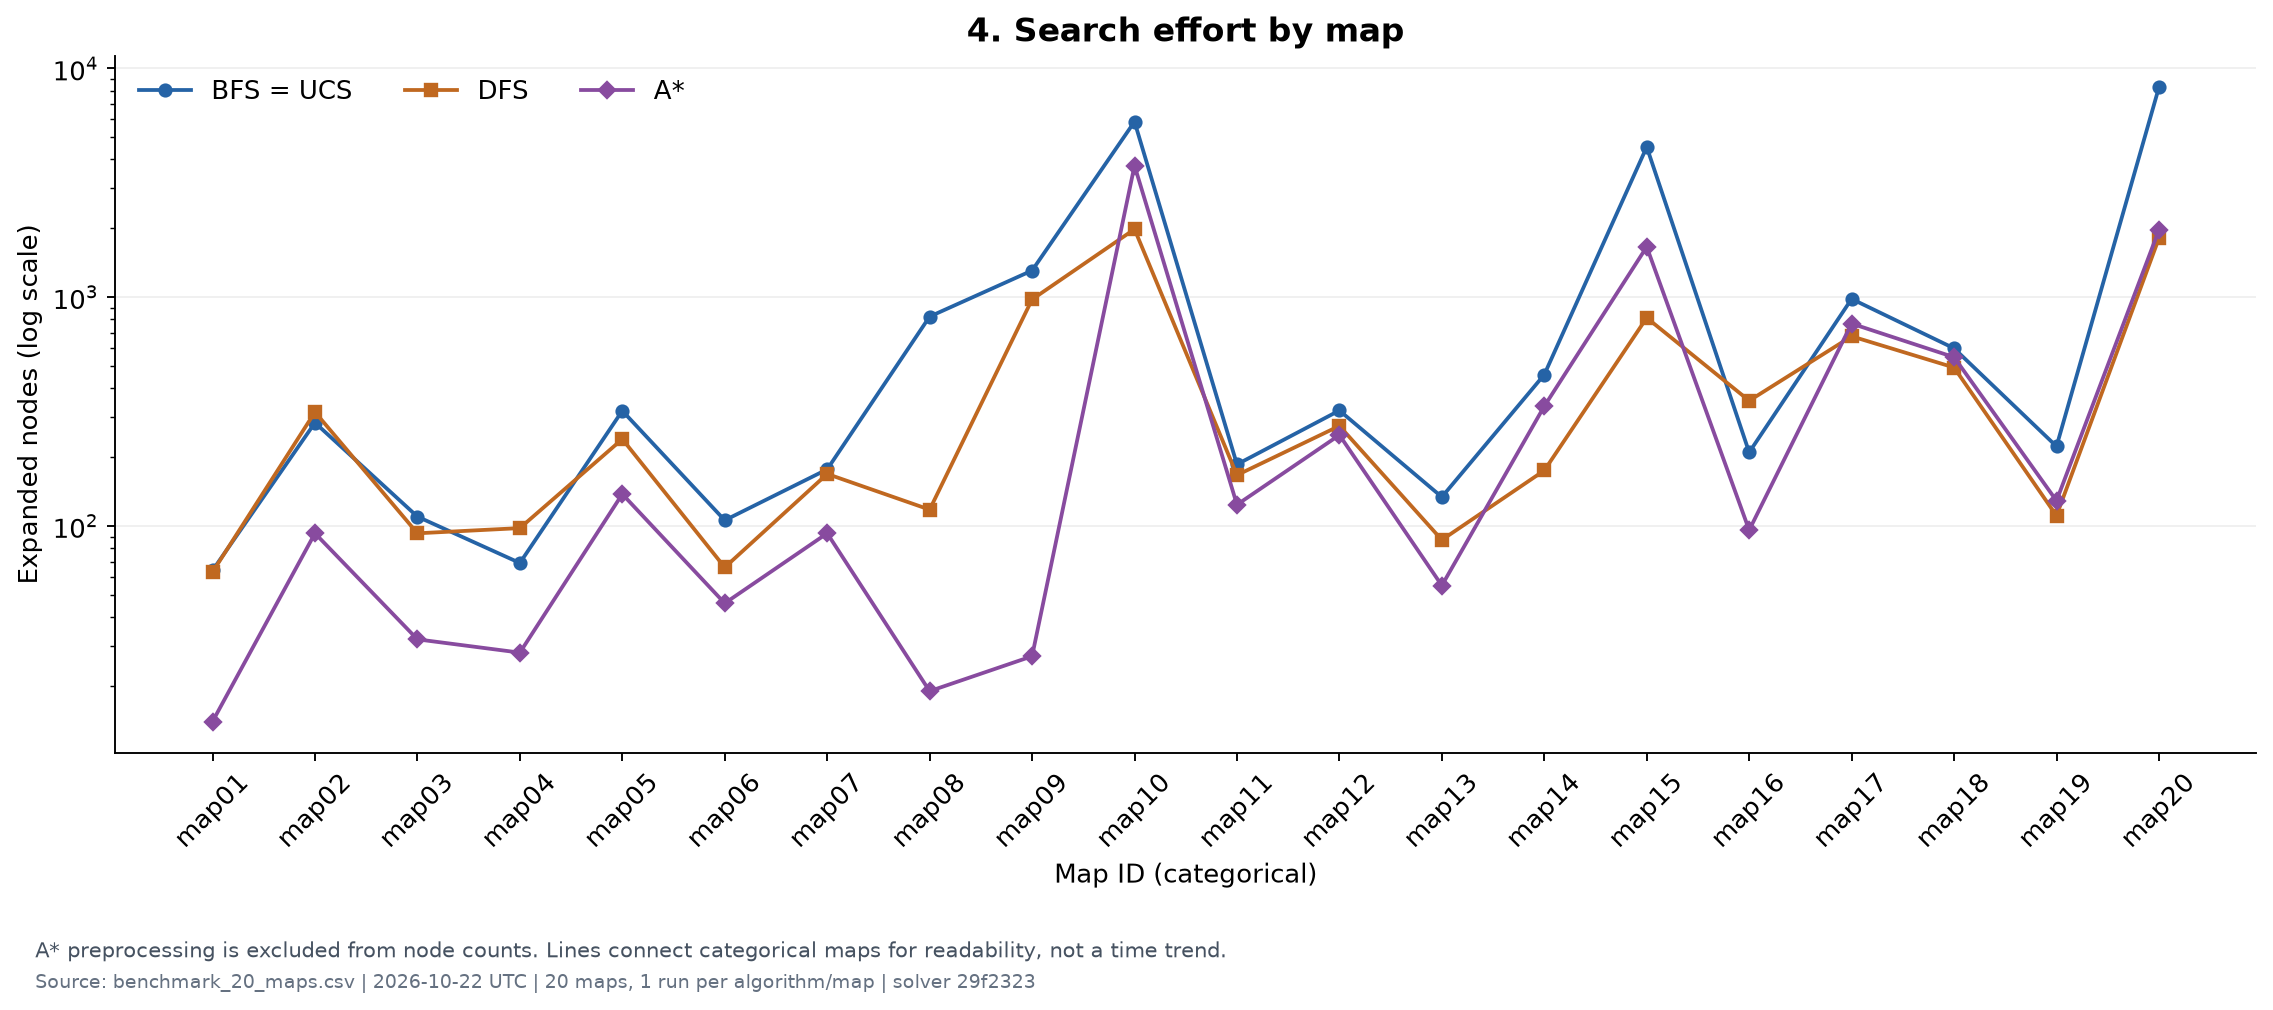
\includegraphics[width=\textwidth]{figures/benchmark_nodes.png}
    \caption{Node mở rộng trên 20 maps. Hai chuỗi BFS và UCS trùng
    nhau trong dữ liệu nên được gộp thành một đường. Nguồn: CSV tại
    commit solver \texttt{29f2323}.}
    \label{fig:benchmark_nodes}
\end{figure}

\begin{figure}[p]
    \centering
    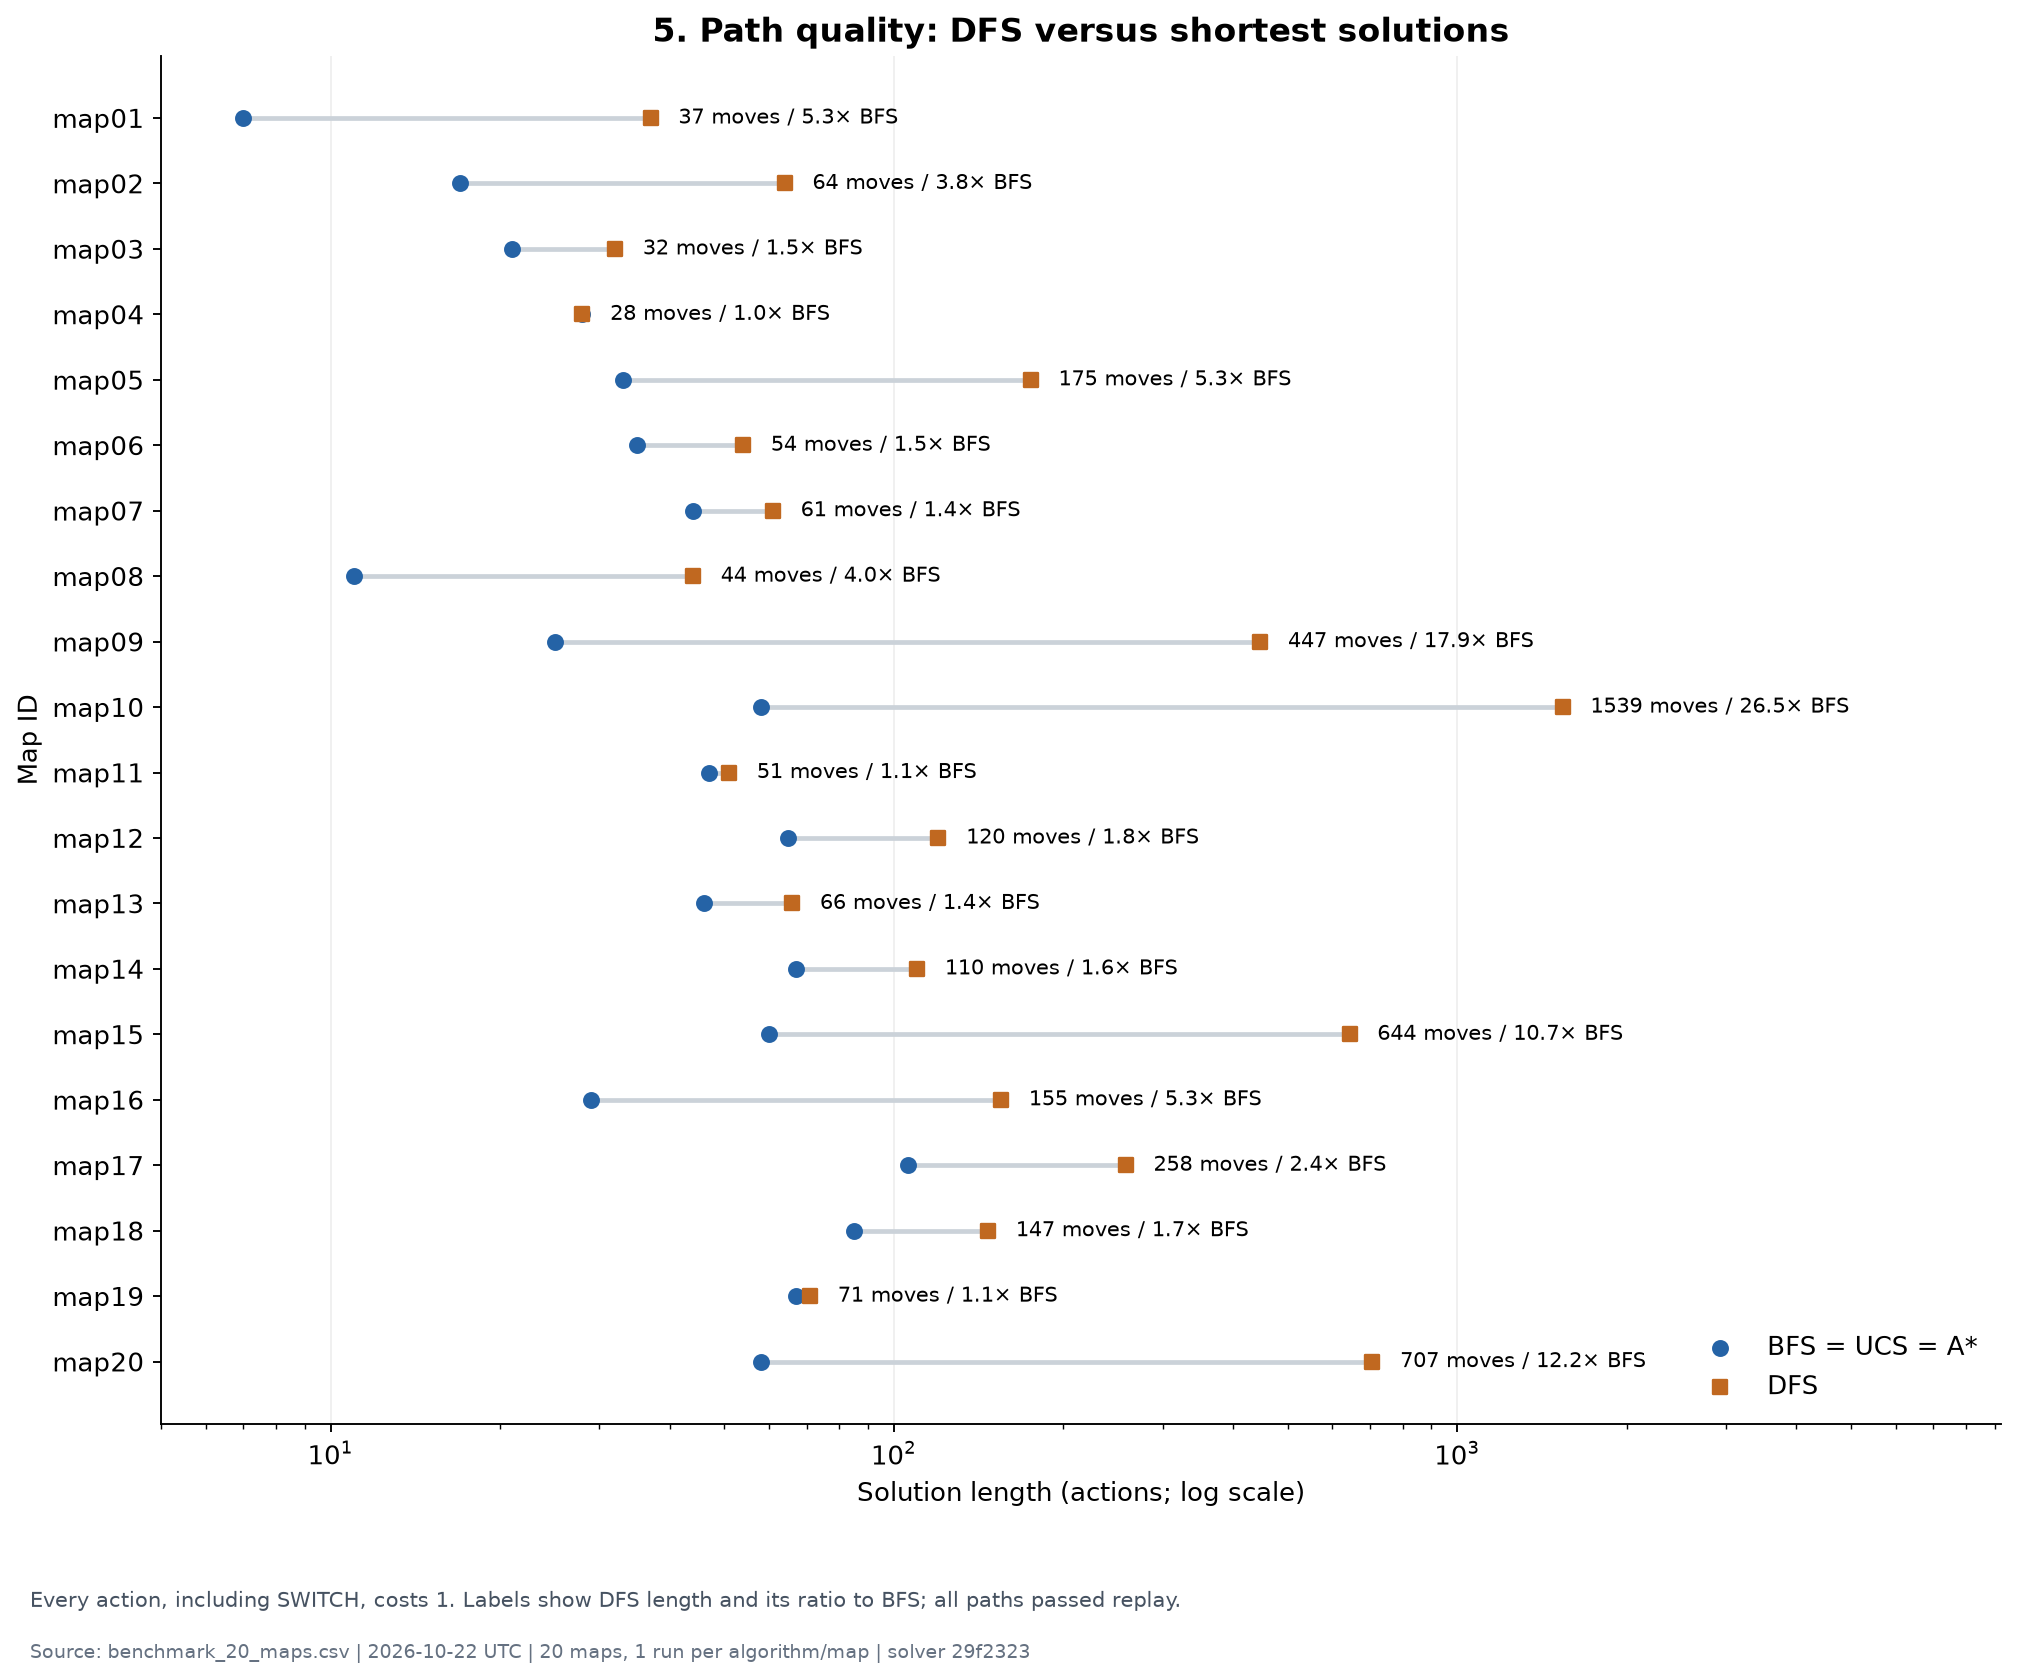
\includegraphics[width=\textwidth,height=0.73\textheight,keepaspectratio]{figures/benchmark_lengths.png}
    \caption{So sánh độ dài lời giải DFS với BFS/UCS/A* trên 20 maps.
    Trục số hành động dùng thang log; hệ số thể hiện số bước DFS chia
    cho số bước BFS trên cùng map.}
    \label{fig:benchmark_lengths}
\end{figure}

\begin{figure}[p]
    \centering
    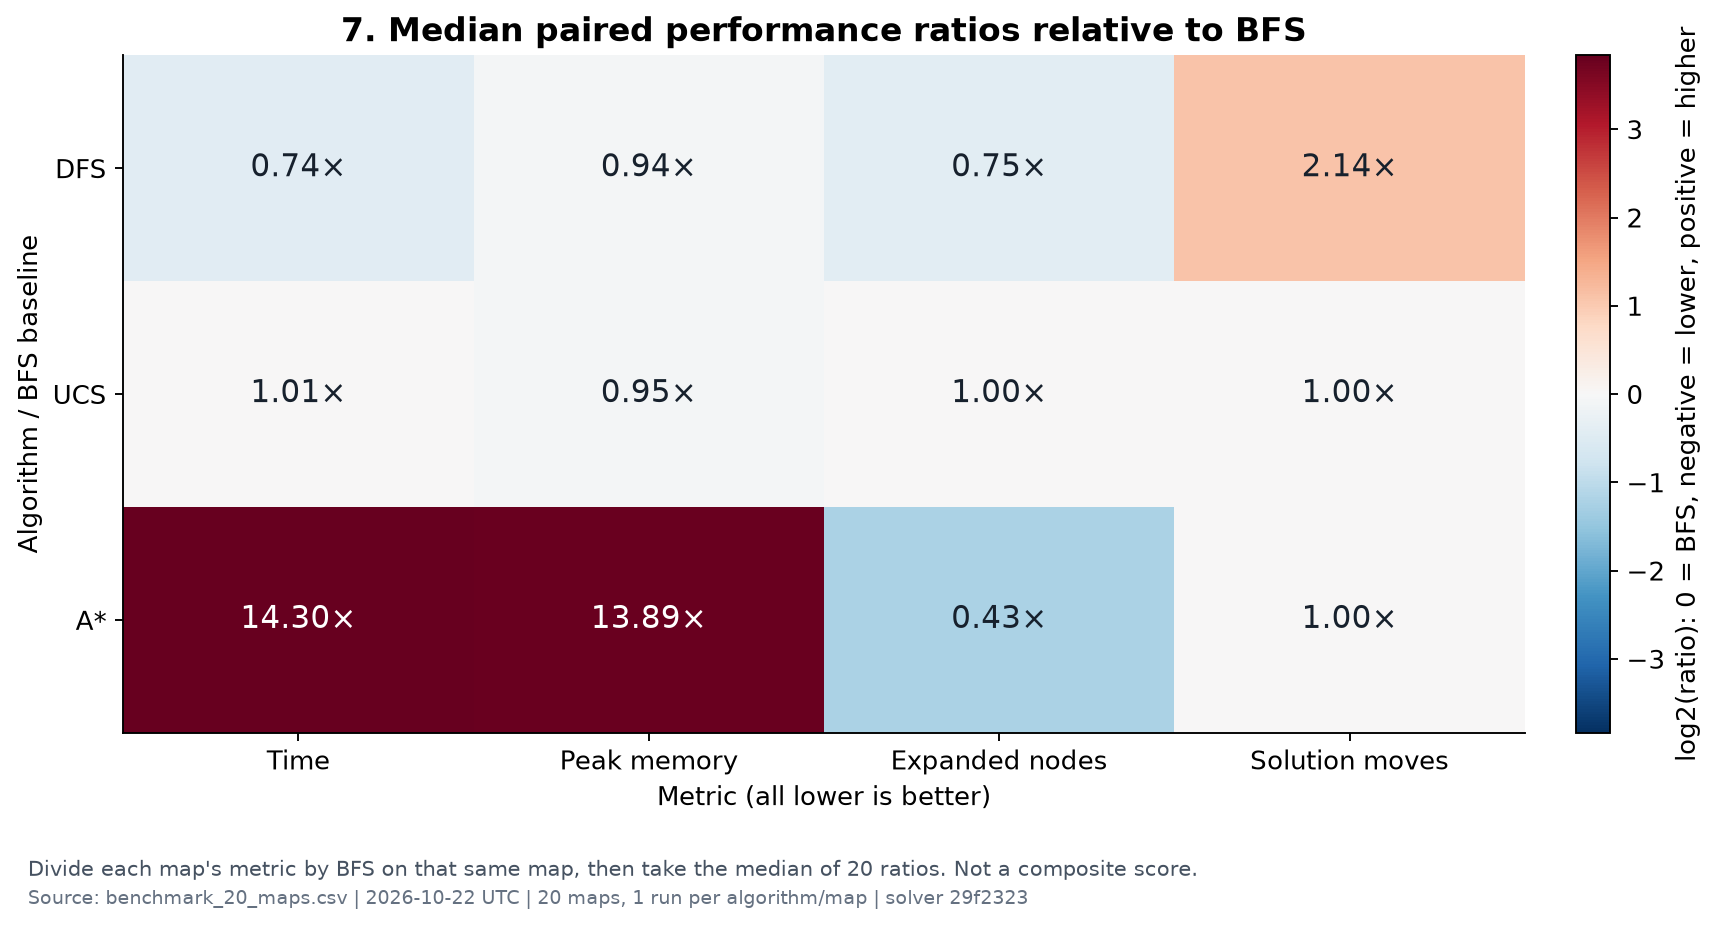
\includegraphics[width=\textwidth]{figures/benchmark_ratios.png}
    \caption{Trung vị tỷ lệ theo từng map so với BFS. Giá trị 1 là
    bằng BFS; thấp hơn 1 là nhỏ hơn ở đại lượng tương ứng. Màu dùng
    thang log cơ số 2 để biểu diễn tỷ lệ.}
    \label{fig:benchmark_ratios}
\end{figure}

\subsection{Hạn chế và hướng mở rộng}

Mỗi cặp map--thuật toán chỉ có một lượt đo nên chưa thể đánh giá độ
ổn định hoặc xây dựng khoảng tin cậy về thời gian. Chênh lệch nhỏ giữa
BFS và UCS không đủ để kết luận ưu thế hiệu năng tổng quát. Boxplot
hiện mô tả sự khác nhau giữa các maps, không mô tả nhiễu qua nhiều
lần chạy cùng đầu vào.

Các bước tiếp theo phù hợp là lặp lại phép đo trên cùng phiên bản
code, lưu số thứ tự trial, thay đổi thứ tự chạy để giảm ảnh hưởng
thứ tự, và tách thời gian dựng heuristic khỏi thời gian tìm kiếm khi
cần phân tích sâu A*. Nếu đo thêm RSS hoặc thay đổi ý nghĩa các cột,
cần bổ sung đại lượng hoặc nâng phiên bản schema thay vì ghi đè ý
nghĩa của số liệu hiện có.
\clearpage
